\chapter{Introduction}
\label{chap:intro}

Computer systems do not operate in a single moment. They execute across time, and their ability to function correctly must hold from the first cycle to the last. A system begins execution in a defined initial state, but as operations accumulate and memory is accessed repeatedly, the likelihood of deviation from intended behavior increases. Every computation depends on fetching instructions and reading or writing data, and each access introduces the possibility of corruption. Reliability therefore is not simply about beginning correctly; it is about remaining correct until the task has completed. Programs that run longer, access more memory, or execute more instructions experience greater exposure to potential failure. A system must maintain coherent operation from its initial state at startup through all subsequent steps, and instability at any point before completion can prevent it from achieving the intended outcome.

The earliest moments of execution are particularly sensitive. At power-on, the system begins running initialization code that transitions it from reset into a usable operating context. During this phase, the processor first consumes instructions and data without yet having confidence in their correctness. Any disturbance in these initial accesses, whether to instruction bytes or configuration values, can disrupt progress, corrupt early state, trigger repeated resets, or halt execution before meaningful work begins. The system therefore starts in an \emph{unqualified memory state}, and its primary challenge is to advance far enough to establish a \emph{qualified memory state} in which continued execution can proceed with a high likelihood of correctness. Until that transition occurs, each memory access carries elevated risk, and failure can prevent the system from ever reaching stable operation.

The central challenge, and the focus of this work, is to increase the probability that a system reaches a qualified memory state even in the presence of memory upsets, mutations, or corruptions. The methods developed here aim to raise the likelihood that early execution continues long enough to establish stability and transition into a trusted operating mode. In effect, the problem is one of \emph{bootstrapping reliability}: enabling a system to move from an unqualified memory state into one where execution can proceed with confidence, despite the possibility that some stored instructions or data differ from their intended form.

\section{Background}
\label{sec:background}

Ensuring long-term system dependability requires mechanisms that limit the impact of memory corruption as it accumulates over time. These mechanisms fall into two broad categories: hardware techniques built into the platform and software techniques applied above the architecture. Hardware mechanisms operate continuously and transparently, reducing error rates within the bounds anticipated by the system design. Software can complement these defenses by providing additional resilience when faults exceed those bounds or occur in regions not fully protected by hardware. Together, these layers form the basis for sustained reliable operation.

\subsection{Hardware-Based Approaches}

Hardware reliability features are intended to preserve stable behavior in the presence of physical memory faults. These capabilities are implemented in memory structures, processor pipelines, and interconnects, and operate automatically at runtime. When fault rates remain within the system's assumptions, hardware can significantly limit the likelihood that corrupted values propagate into execution.

Error-correcting codes (ECC) detect and correct a bounded number of bit flips by storing additional redundancy alongside memory words. Memory scrubbers may proactively scan memory to repair correctable faults before they accumulate. As long as errors stay within the correction capacity, memory reads continue to reflect their expected values.

Lock-step execution provides another protection strategy by running identical instructions on multiple processor cores and comparing outputs cycle-by-cycle. Divergence between the cores signals a fault and prompts error handling or safe shutdown. Such mechanisms are common in high-assurance settings where correctness is prioritized over resource cost.

These techniques significantly reduce error exposure but operate within finite design margins. ECC corrects only a limited number of bit errors; beyond that boundary, corruption may escape detection or propagate silently. Lock-step execution detects computational divergence but does not prevent slow accumulation of corruption in instruction or data memory. Over long deployments, persistent or gradually accumulating memory faults may eventually exceed hardware protections. At that point, additional layers must assist in preserving dependable execution.

\subsection{Software-Based Approaches}

Software techniques provide a second line of defense when memory integrity cannot be fully guaranteed by hardware alone. Unlike physical redundancy mechanisms, software methods require no special fabrication or memory features and can be deployed on existing platforms at compile time or runtime. Their purpose is to manage execution behavior when faults occur, increasing the likelihood that the system continues to operate correctly or fails in a controlled manner.

Two broad strategies are used: detection and recovery.

\begin{itemize}
  \item \textbf{Detection} identifies when program behavior deviates from expectations. It may take the form of consistency checks on control flow, validation of stored values, or cross-checking between redundant computations. Detection does not directly correct state; it provides awareness that an upset has occurred so the system can react deliberately instead of unknowingly propagating corruption.

  \item \textbf{Recovery} aims to bias execution toward correct behavior even in the presence of faults. It uses structural or algorithmic redundancy so that when disturbances occur, execution remains aligned with the intended program logic. Recovery may reconstruct values from encoded representations, select among multiple candidate results, or apply transformations that preserve expected semantics. Rather than responding only after failure, recovery increases the probability that execution continues along a valid trajectory despite disturbances.
\end{itemize}

While hardware techniques provide essential protection against memory disturbances, they cannot always ensure correct execution over long operational lifetimes, especially as stored state gradually mutates or exceeds correction limits. Software mechanisms offer a complementary path: they operate above the physical substrate and can be deployed without modifying the underlying hardware. Because they can be adapted, tuned, or introduced at any point in a system's lifetime, software-based approaches can reinforce execution even when hardware protection is minimal or aging.

Software reliability techniques broadly pursue two goals: recognizing when execution deviates from expectations and increasing the likelihood that execution remains correct despite disturbances. Together, detection and recovery can significantly improve reliability by identifying inconsistencies and maintaining forward progress in spite of faults. These methods do not depend on hardware configuration or fabrication constraints and can therefore extend reliability beyond the limits of physical memory protection. In this work, we focus on software-based mechanisms that increase the probability a system reaches and maintains a stable operating state, even as memory content mutates over time.

\subsection{Related Work}

Software reliability techniques typically harden either the data path, the instruction path, or both. These approaches work by controlling how memory is used and verified so that stored and computed values remain aligned with intended program state, even when memory disturbances occur.

\textbf{Data-path hardening} ensures that values stored in and loaded from memory remain correct. A widely used approach is \emph{shadow memory}, where each memory region is replicated in one or more shadow regions. On every load, the system retrieves values from all replicas and resolves them through a convergence filter that biases execution toward the intended value. On every store, all copies are updated in parallel, maintaining structural alignment across regions. When a disturbance affects one location, the replicated layout prevents error amplification and maintains consistent state. Other methods use encoded computation, such as AN-codes, to detect mutations by embedding arithmetic structure into stored values.

\textbf{Instruction-path hardening} protects the control and execution flow. Control flow checking assigns lightweight signatures to basic blocks and verifies them at entry to detect illegal jumps or unexpected transitions. Execution redundancy replicates dependence chains and compares computed results at runtime. Deviations indicate incorrect behavior and lead to recovery or controlled halt, maintaining expected program direction and correctness during execution.

Some systems combine both instruction and data protection. \emph{SWIFT-R} is one example, integrating replicated execution chains with shadow memory to reinforce correctness across the entire execution pipeline. This coupling increases resilience by ensuring that both the data state and the execution trajectory remain consistent, even when memory upsets occur.

Most state-of-the-art reliability mechanisms rely on a \emph{post-execution detection strategy}, where faults must first occur before they can be recognized and recovered. This model works reasonably well for data, since corrupted values can often be detected or corrected after they are read. For instructions, however, this assumption becomes a critical limitation. If corrupted instructions must execute in order to trigger detection or recovery, the system may already have lost control flow or corrupted its internal state beyond repair. Furthermore, many instruction-hardening schemes increase fault exposure indirectly: by duplicating or triplicating dependence chains, they inflate the instruction stream and expand the portion of memory that must remain fault-free for recovery logic to function. As a result, mechanisms intended to improve resilience can inadvertently reduce the probability of successful recovery.

This work instead focuses on \emph{pre-execution validation}, seeking to identify and neutralize corrupted instructions before they are executed. The goal is to raise the probability that early execution proceeds through trustworthy code regions, allowing the system to reach a stable, qualified state even when underlying memory contains latent upsets or mutations.

A practical example of pre-execution validation already exists in the form of the \emph{A/B image strategy} used in many embedded ARM systems. This method maintains two complete firmware images—designated A and B—stored in non-volatile memory. During boot, the system inspects each image and selects one to execute based on integrity checks or update status. Although primarily designed for safe firmware updates, this mechanism inherently supports fault tolerance. If both images are functionally identical, one can serve as a verified fallback when corruption is detected in the other. The same concept can be extended beyond two images—maintaining multiple replicas increases the probability that at least one remains uncorrupted and executable. By validating and selecting the execution target before any instruction is fetched, such multi-image schemes satisfy the principle of pre-execution validation: code is qualified prior to use, and execution proceeds only from trusted regions of memory.

The progression of these techniques reflects a shift toward proactive reliability, qualifying code and data before they are executed rather than responding after faults occur. Replication-based methods, such as multi-image validation, demonstrate one way to achieve this early assurance. The following section introduces another perspective, comparing replication with repair as complementary strategies for establishing qualified memory before execution begins.

\section{Replication vs. Repair}
\label{sec:replication-vs-repair}

Replication and repair represent two complementary strategies for maintaining reliable operation in the presence of memory upsets.

Replication preserves multiple functionally identical variants of code or data and selects among them at runtime. The granularity can range from entire program images to individual bytes. Below the image level, access must pass through a layer of indirection: a lookup table holds references to valid replicas, and all reads or calls are routed through this table. For data, each memory operation is redirected through the table so that loads and stores target a qualified copy. For instructions, calls and branches entering or leaving a protected region are resolved through the same indirection mechanism, ensuring execution proceeds only through verified variants.

Repair, in contrast, operates in place. Rather than selecting among alternatives, it reconstructs or corrects corrupted memory directly. Proactive repair can resolve faults down to the bit level without altering the instruction stream. It depends on two main design factors: redundancy and complexity. Redundancy provides the extra information needed to restore the original state, while complexity determines the time and code cost of performing that restoration. Together, these form a three-way trade-off among redundancy, computational effort, and achievable reliability.

At finer granularity, repair typically outperforms replication. Replication requires that every bit in the protected region remain correct in at least one copy; any corruption in all replicas of the same position leads to failure. Repair, by contrast, uses available redundancy to reconstruct missing or altered information, making more efficient use of stored data. Because of this, repair should be applied as soon as the system environment allows modification or rewriting of memory. The next section examines how system constraints influence the choice and timing of each strategy.

\section{System Architecture and Memory Constraints}
\label{sec:system-architecture}

System architecture plays a central role in determining which reliability strategies can be applied and how effective they are. The nature of the memory hierarchy, including its volatility, accessibility, and organization, defines the practical limits of replication and repair.

Dynamic memory elements, including caches, registers, and RAM, are volatile by design. Their contents are cleared after each power cycle, which naturally removes any accumulated corruption. In such memory, recovery mechanisms focus primarily on detection. Once corruption is identified, a reset or reinitialization can restore correct state without permanent loss. Persistent protection is therefore less critical, since faults do not survive across reboots.

Static memory, in contrast, retains its contents across power cycles and exists in both writable and read-only forms. Repair requires write access, which makes it infeasible for regions that are permanently locked or physically read-only. Writable static memory, such as flash, introduces additional constraints. Flash memory cannot be read and written simultaneously within the same region and requires a program--erase (P/E) cycle to modify data. As a result, code responsible for repair cannot safely reside in the same section that is being rewritten. For instruction repair, coherence hazards may also arise if cached instruction data is modified without appropriate synchronization. These conditions are typically managed by hardware mechanisms that support self-modifying code but impose strict operational ordering.

Memory organization also shapes the feasibility of both replication and repair. Figure~\ref{fig:harvard-von-neumann} compares the Harvard and Von~Neumann architectures. In a Von~Neumann architecture, instructions and data share the same address space, allowing software to generate or modify executable code dynamically. This flexibility supports both instruction and data repair at runtime. In a Harvard architecture, instructions and data reside in physically separate memory spaces. Stores cannot target instruction memory, restricting repair to data regions only. While this separation improves security by preventing unintended code modification, it also prevents in-place instruction repair.

\begin{figure}[t]
  \centering
  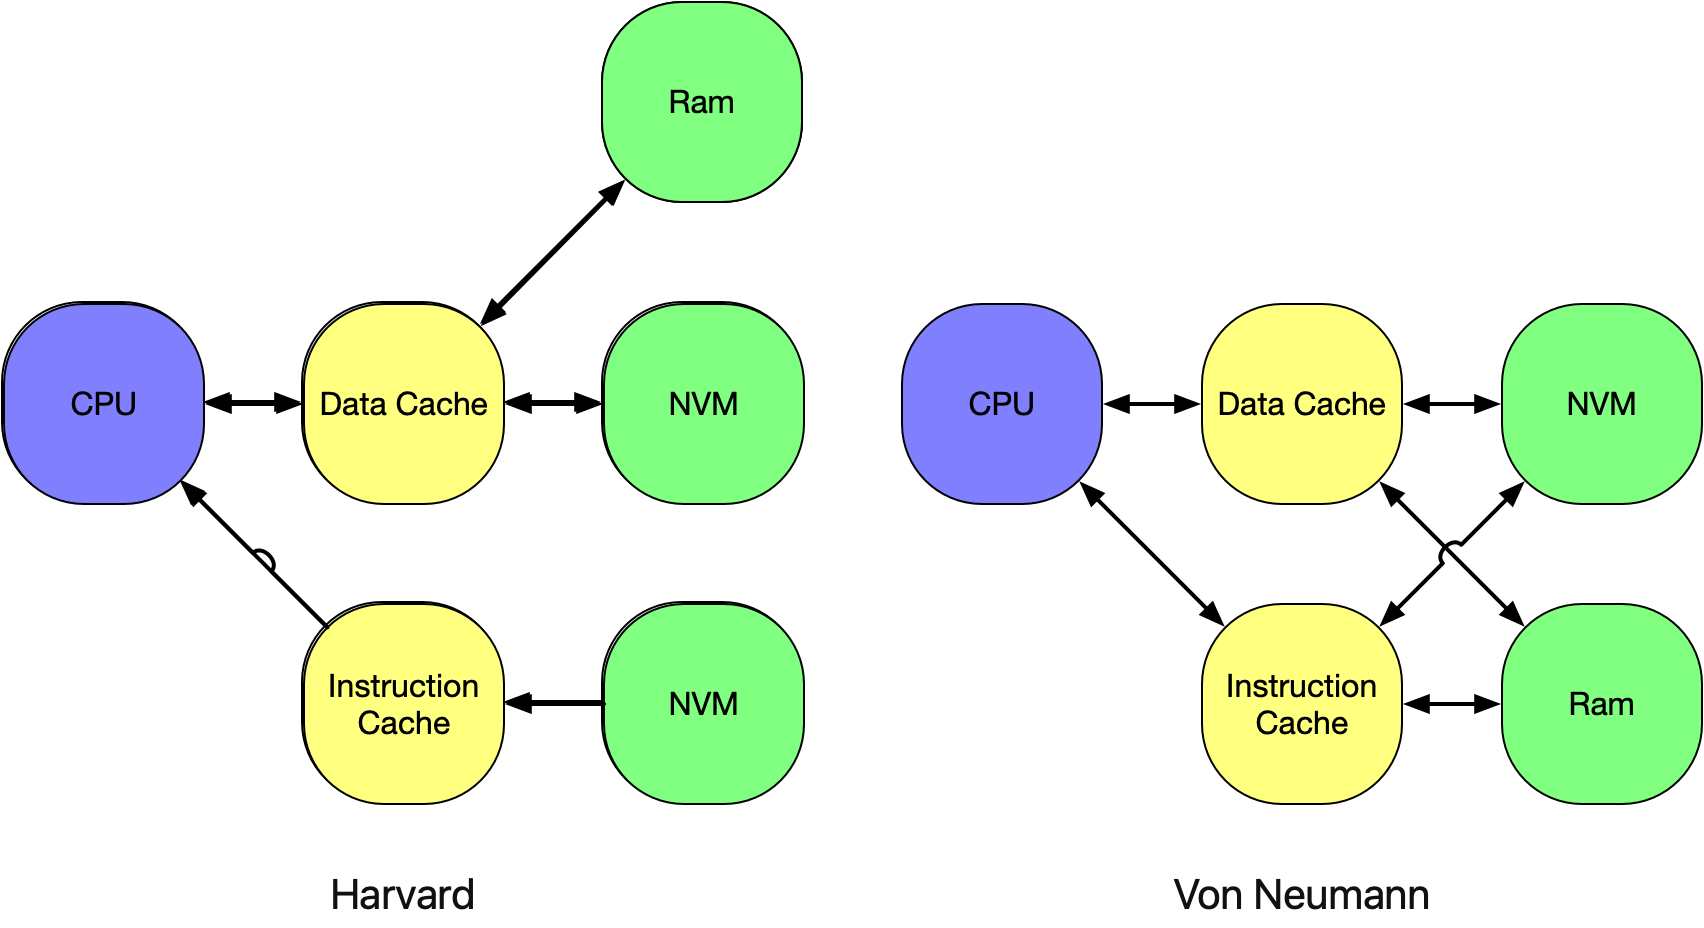
\includegraphics[width=0.9\linewidth]{Chapter-1/figs/HarvardxVon.png}
  \caption{Comparison between Harvard and Von~Neumann architectures. Harvard systems maintain distinct physical memory paths for instructions and data, improving security and predictability but preventing runtime modification of instruction memory. Von~Neumann systems share a unified address space, allowing both instructions and data to coexist and be modified dynamically, enabling flexible software-based repair but introducing potential reliability risks from shared corruption sources.}
  \label{fig:harvard-von-neumann}
\end{figure}

Hybrid architectures combine elements of both. They maintain separate instruction and data spaces for security-critical components while allowing writable or unified memory for dynamic regions. In hybrid designs, read-only sections are a deliberate design decision. In most embedded systems, execution proceeds in two phases: a read-only bootloader stored in ROM and a writable bootloader stored in flash. Some systems include internal flash memory on-chip that can control which medium or image is used for the next boot phase. These mixed designs require selective application of reliability mechanisms, using replication for immutable instruction areas and repair for writable data and code regions where modification is permissible.


\section{Motivation and Focus of This Work}
\label{sec:motivation}

The distinction between dynamic and static memory defines where reliability mechanisms can operate effectively. Dynamic memory is inherently recoverable: its contents are volatile, and corruption can be cleared simply by resetting the system or refetching data from a trusted source. Post-execution validation methods therefore work well in this domain, and extensive research has established effective strategies for detecting and correcting transient faults.

Static memory, by contrast, retains its contents across resets, making it a long-term source of unrecoverable faults. Errors in these regions persist and reappear every time the program executes. Figures~\ref{fig:section-breakdown-m2} and~\ref{fig:section-breakdown-embedded} show the normalized composition of representative binaries collected from an Apple-based general-purpose system and an Arduino-class embedded processor. In both cases, the majority of bytes reside in the \texttt{.text} section, which contains executable instructions. The \texttt{.rodata} and \texttt{.data} sections, while smaller, are mutable or copyable into RAM during initialization and can therefore be repaired using conventional techniques. Instruction memory, however, dominates the static footprint and cannot be trivially rewritten or refreshed once execution begins.

This gap defines the central focus of this work. While data reliability is well understood and broadly supported by existing software and hardware mechanisms, instruction reliability remains a critical weakness. The remainder of this thesis evaluates two complementary strategies for improving the survivability of instruction memory: \textbf{replication}, which provides multiple alternate copies for redirection, and \textbf{repair}, which reconstructs corrupted code in place. Together, these approaches aim to increase the probability that execution can continue successfully even when faults occur in static program storage.

\begin{figure}[t]
  \centering
  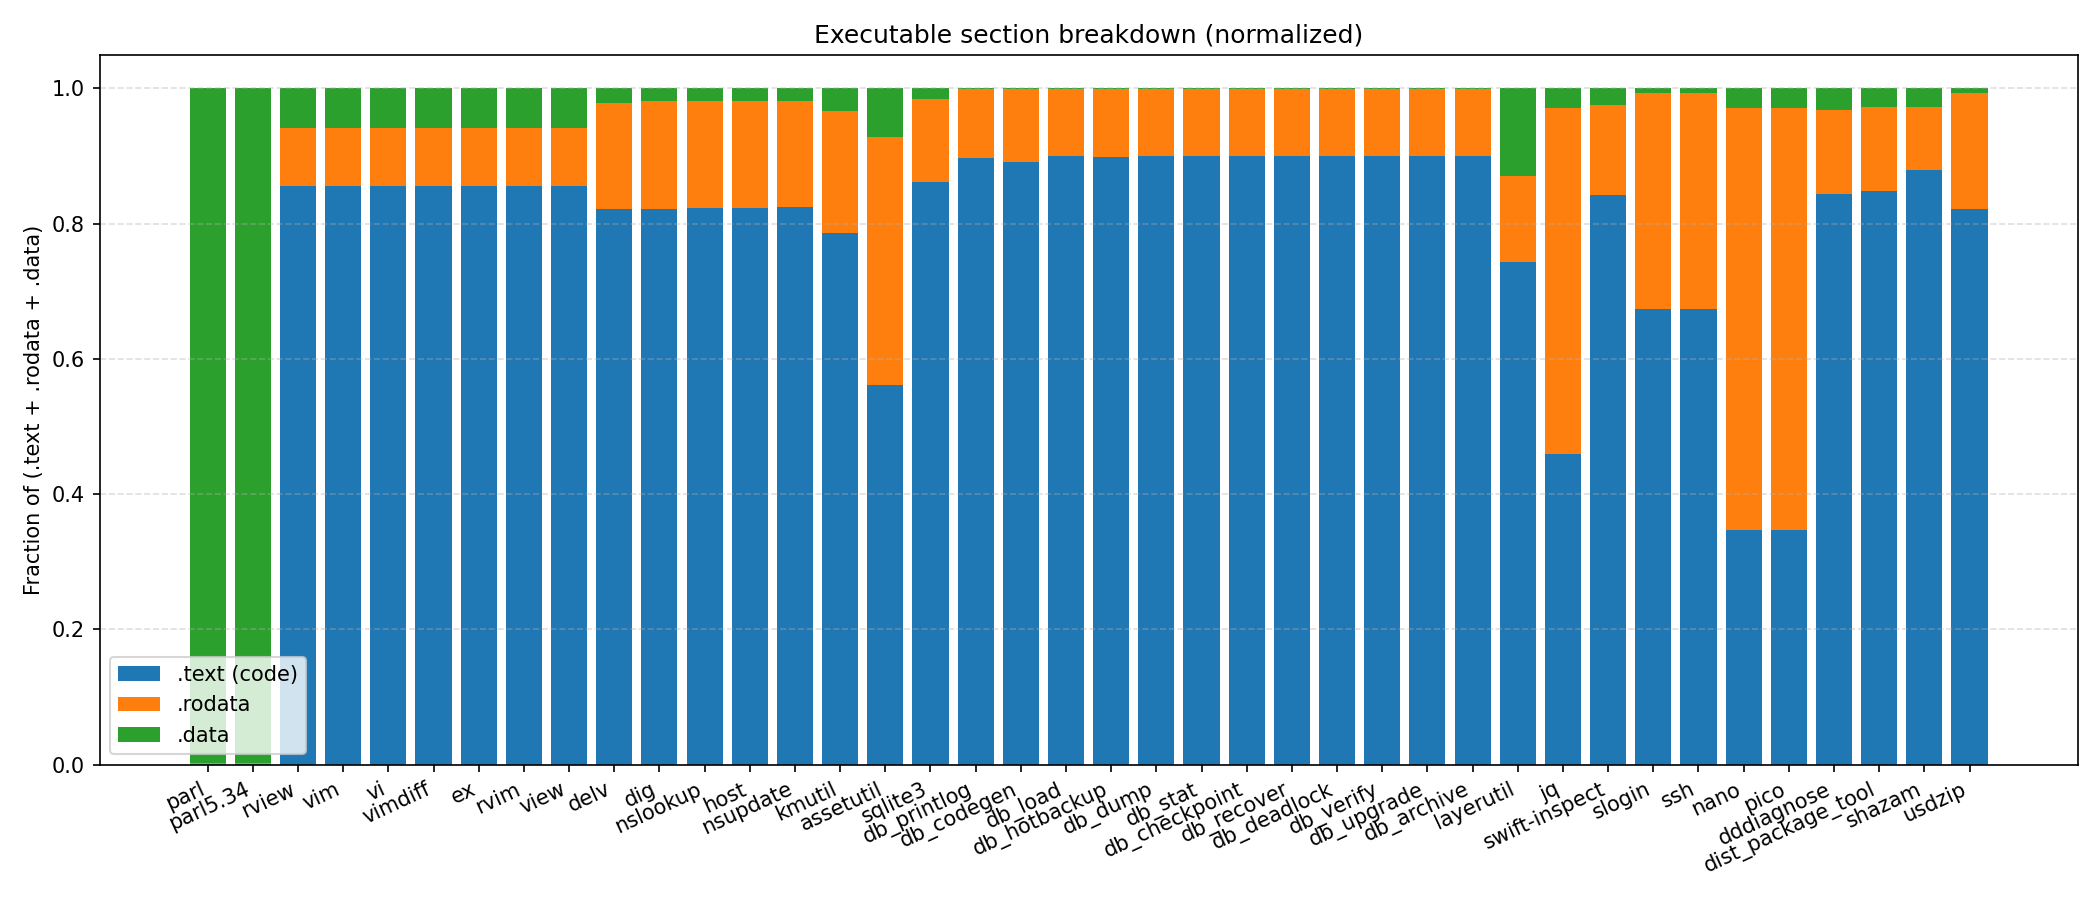
\includegraphics[width=0.9\linewidth]{Chapter-1/figs/apple-bin.png}
  \caption{Executable section breakdown of representative user-space binaries compiled for an Apple-based general-purpose system. The \texttt{.text} section dominates the static footprint, with \texttt{.rodata} and \texttt{.data} contributing smaller fractions.}
  \label{fig:section-breakdown-m2}
\end{figure}

\begin{figure}[t]
  \centering
  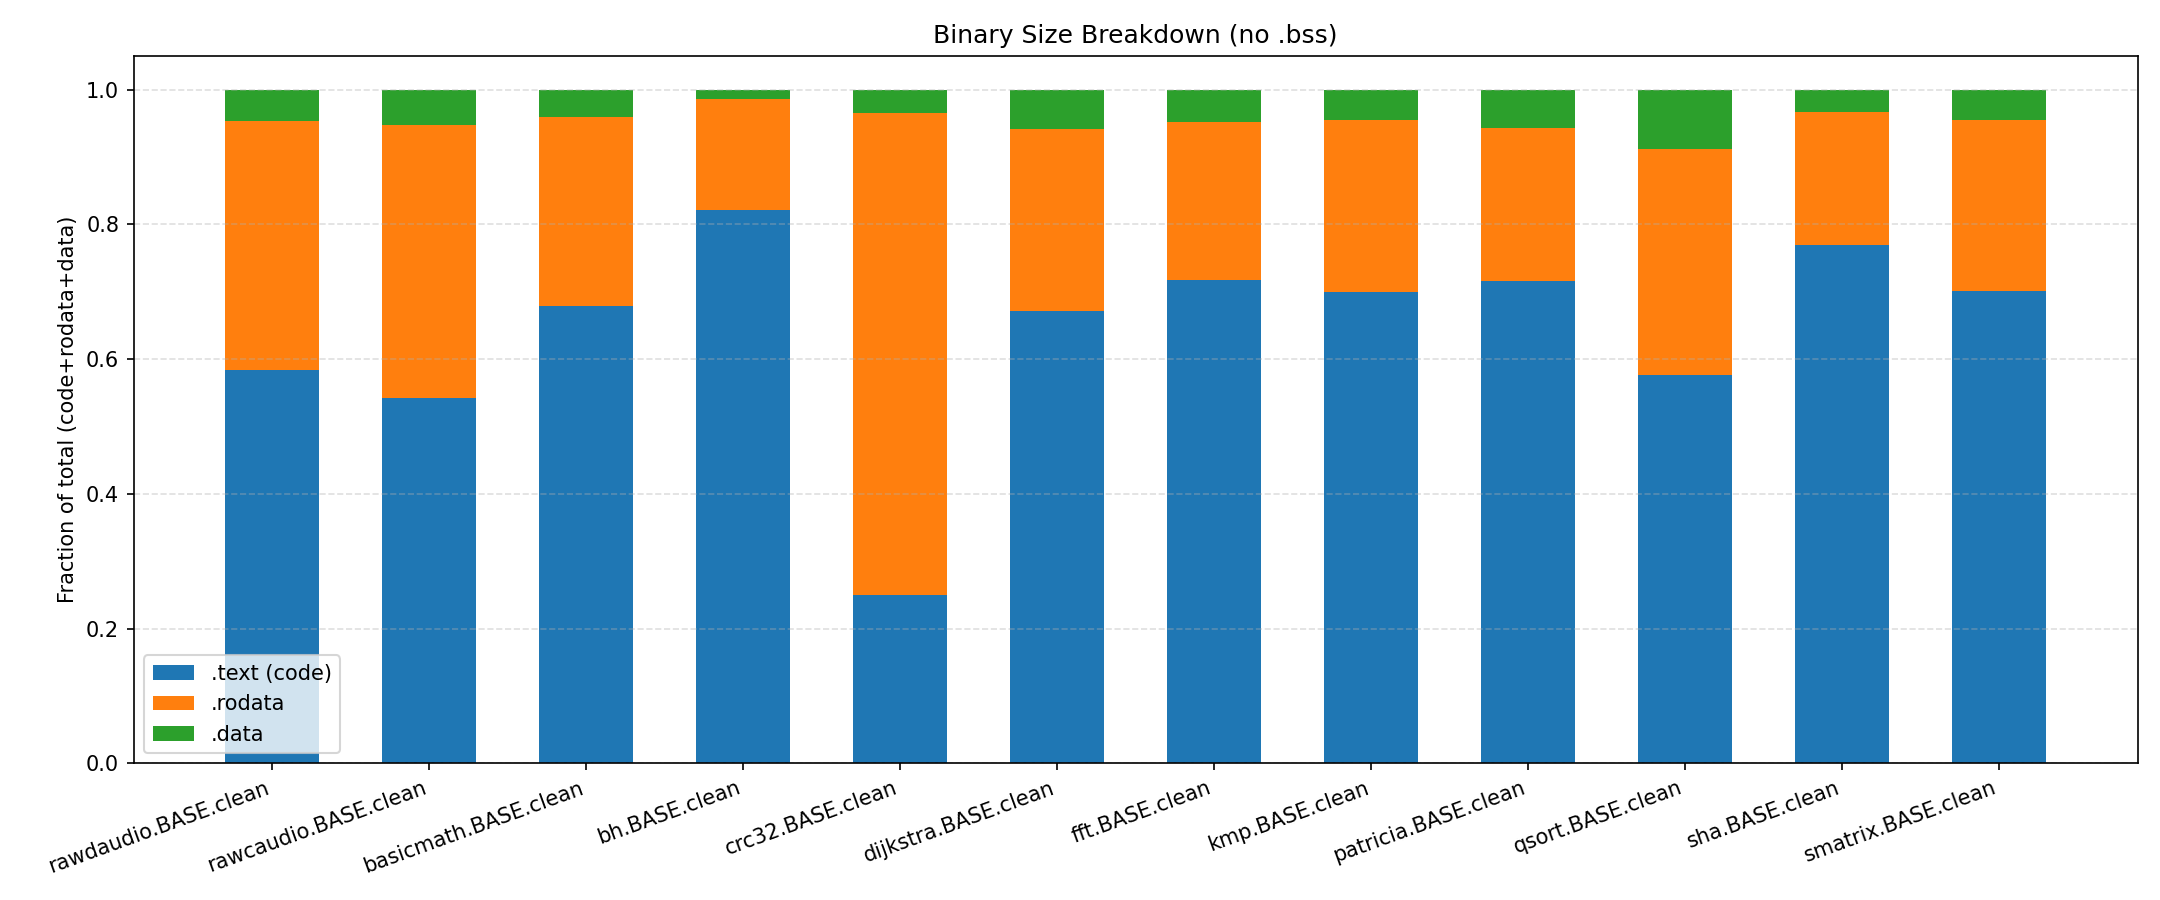
\includegraphics[width=0.9\linewidth]{Chapter-1/figs/embedded-bin.png}
  \caption{Executable section breakdown of representative embedded benchmarks compiled for an Arduino-class processor. Similar to general-purpose systems, code regions dominate the static memory footprint.}
  \label{fig:section-breakdown-embedded}
\end{figure}